\title{Reconstruction of strange attractors via inter-spike intervals}
\author{\`Alex Arcas Cuerda \& Ram\'on Marc Garcia Seuma}
\date{\today}
\documentclass[10pt]{article}

\usepackage[a4paper, total={7in, 10in}]{geometry}
\usepackage{graphicx}
\usepackage{amsmath}

\begin{document}
\maketitle

\section{Introduction}

We choose these papers because when we both read them we found them really interesting for different aspects. 

One, and probably the most surprising and interesting for both because we didn't know it, the fact that chaotic systems could be reconstructed using time series of \textit{any} of the independent variables of the system. This was at first glance really anti-intuitively and it's actually been hard to understand it.

Then, we also enjoyed the background and the applications they gave in the papers, we found great to know that these were the papers introducing these concepts for first time and that they would hypothesize with their applications with fluids systems and biological systems, topics in which we are interested and working.

Finally, it was more like an anecdote but it was funny to read the paper once and twice and notice that they were really \textit{different} to what we're used nowadays. The papers, although really important and from important universities, lack of good mathematical proves and were more what we would say '\textit{bla bla bla}' than really science in a sense we would understand today. Both give some great intuition in their topics and when addressing scientific formality, first is far less formal.

Is mainly for these ideas that we chose these papers and we can now gladly say that we've happy to have chosen them as we've learned a lot and we liked them too.

\section{Geometry from a Time Series}

\subsection{Summary}

The idea of \cite{paper1} is to give some insight in turbulent or chaotic systems. To do so, they enfatice that the usual data in this experiments is some observable of the system sampled at regular times. 

First, they show the fact that one can reconstruct the topology of such a systems just with one coordinate of any dynamical system. Really, what they show is that one can reconstruct the topology of the system using any combination of $D$ independent variables of the systems, where $D$ is the dimension of the system. They show that this procedure works for the Rossler attractor.

Then, they show that for a systems with only one positive-characteristic exponent(Liapunov exponent in modern terms), one can extract it just using the description defined above ergo one only needs one coordinate to find the exponent. They compute these exponents with different descriptions for the Rossler attractor and show how well the results fit with the exponent extracted from the 3-coordinate one.

Finally, they state that one can obtain the dimensionality of an attractor from using the description used above. To do so they give a 'general' procedure in which one graphs the conditional probability of a coordinate $x_i(t)$ knowing $k$ previous values, $(x_i(t-\tau), ..., x_i(t-k\tau))$. Then, they state that the $k$ for which the graph displays a peak as sharp as possible, is the dimension of the attractor. They use this to extract that the dimension of the Rossler attractor is two.

\subsection{Review}

We first find this paper really interesting and in fact we still do. Despite, we have some major objections to it. To start with, they don't really \textit{prove} anything they just show that they've found it works that way and they give some examples to support it's hypothesis. Being more precise, they don't show why the topology of the phase space is conserved using their logic so it can all be wrong. In fact, Takens theorems \cite{takens} proves what they conjecture but arguing why the fit is not the dimension of the dynamical system but two times in general. Moreover, the procedure they give to compute the dimension of the attractor it's latter proved to be effective only in really \textit{flat} strange attractors and for the Rossler case it isn't exactly two.

So our final review would sum up that they found some really important intuition about dynamical systems given some \textit{time series} of it but they had much work to do yet. We have to remember that the paper is from 1979 and at that time the knowledge of strange attractors was really poor.

\section{Reconstruction of Dynamical Systems from Interspike Intervals}

\subsection{Summary}

The paper \cite{interspike} tries to pose the following question: being a point process the manifestation of an an underlying deterministic system, it is possible to identify the states of the system from the information provided in those sequence of points? The point process is simply a series of event timings. The main motivation of this question comes from examples found typically in biology, particularly in microbiological systems, where amplitude measurements of an observable, such as neuronal currents, are not possible (nor desirable), but a series of pulses or spikes emitted at certain times are recorded. In the case of the neurons, for example, we normally have the firing times, emitted when the cell reaches a threshold potential, which triggers depolarization and then the cycle is restarted.

On the other hand, they rely on the fact that states of finite dimensional dynamical systems correspond in a one-to-one manner with delay-coordinate vectors, which are vectors of time series measurements of a generic system observable. System analysis of this type is suggested in and an embedding theorem due to Takens established its validity. This has great consequences and applications, because we can analyse topology and even geometry of the chaotic attractor. The applications can be noise filtering, prediction of chaotic time series.

Takens' theorem \cite{takens} is a delay embedding theorem, i.e it gives the conditions under which a chaotic dynamical system can be reconstructed from a sequence of observations of the state of the system. The important point is that the reconstruction preserves the properties of the system that do not change under smooth coordinate changes. Nonetheless, it does not preserve the geometric shape of structures in phase space. The theorem basically states that the strange attractor can be embedded in $k-$ dimensional Euclidean space with $k>2d_A$, being $d_A$ the box counting dimension $d_A$. It is an upper constrain for the dimension needed, but we still can find our dimension to be lower than this, as we see in the Rossler system, we need to take ISI series of dimension 3.

Thus the paper, relying the Takens' theorem, analyse the previous question for inter-spike interval (ISI) data, assuming a generic integrate-and-fire model coupling deterministic dynamical systems to a spike train, so that there is assumed that there is a one-to-one correspondence between the states of the system and the inter-spike interval vectors of sufficiently large dimension. 

Thus they create signals $S(x)$, being $x$ the trajectories provided by the dynamical system described by the Rossler and Lorentz attractors. Then the firing times $T_i$ are inferred recursively by the equation:
\begin{equation}
\int_{T_i}^{T_{i+1}} S(t)dt=\Theta
\end{equation}
Then from $(1)$, the inter-spike intervals are defined as $t_i = T_i - T_{i-1}$. Those intervals can define the ISI vectors $(t_i,...,t_{i-m+1})$, m took in accordance to the Takens's theorem, so that it can be used to reconstruct the attractor $X$. Using different types of signal for the different analysis they perform, they reconstruct a Rossler attractor, but they later focus on the Lorentz dynamics. In order to determine that deterministically driven ISI series can be distinguished from stochastically driven ISI series, they perform a prediction algorithm in the inter-spike intervals obtained from the deterministic system and to some series of what is called surrogate data. They show that there is predictability not explained by any of the null hypotheses controlled for by the surrogate data. As the threshold $\Theta$ increases, predictability of the series decreases. They also analyse the effect of lengthening the prediction horizon, showing that there is several-step-ahead predictability in the original ISI series.

\subsection{Review}

There are several points that seems to have a lack of purpose or explanation in the paper. They seem to take specific signals, apparently arbitrary, although they specify it is obviously needed positive signals in order to have spike events. They just reconstruct the Rossler attractor (they also write wrong the equations of this dynamical system), and give no explanation on why the Lorentz one its not observable from the spike interval time. They also fix the embedding dimension $m=3$, giving little explanation. So we had the feeling that most of the calculations and parameters are taken to confirm the results; although they claim at the beginning of the paper that their goal is to develop a model which is as generic as possible, their choices are not well justified, and there are some points that can not be fully understood by simply following the paper even the references. Nevertheless, it shows interesting results that seem to have important implications and we were able to reproduce its most important results with the parameters given by them.

\section{Results}

Now we present all the results we reproduced from the papers reviewed above. We basically analyse and compute characteristics of the Rossler and Lorentz systems using the new techniques that both papers gave at their time.

First, we reconstruct a finite-dimensional phase-space picture of the sampled system's time evolution, corresponding to the Rossler equations. We've reconstructed the system using the variable systems they propose in \cite{paper1}. Apart from that, we didn't go further on with reproducing the results of this paper as we thought second one was more interesting and we didn't really agree with the other results in \cite{paper1}. The reconstructions are shown in Figure 1, where one can appreciate how although computed in $2d$, the systems seem just a perspective of a $3d$ system. That is of course consequence of our description with two variables.

\begin{figure}[h!]
\centering
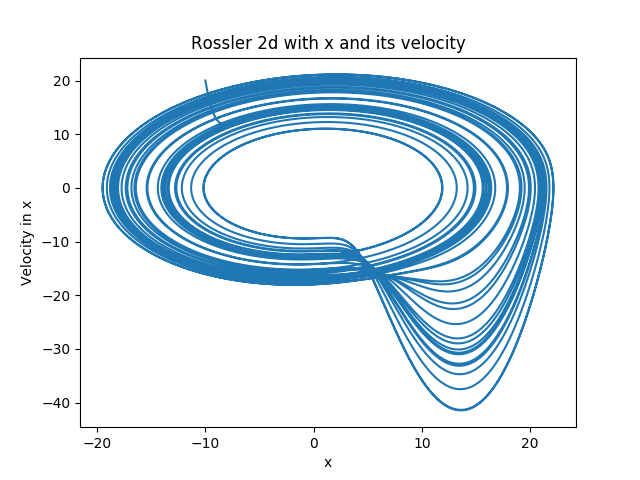
\includegraphics[scale=0.45]{rossler_x_xprima.png}
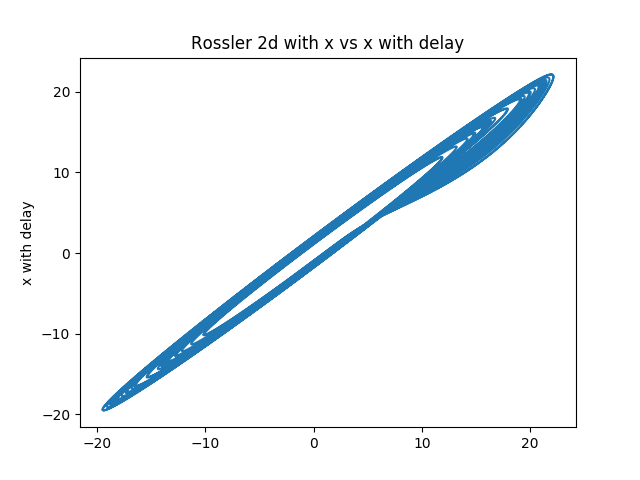
\includegraphics[scale=0.45]{rossler_x_xdelay.png}
\label{fig:rossler_x_xprima}
\caption{Reconstruction $(x,\dot x)$ left and $\left(x(t),x(t-\tau)\right)$ right from the time series for the Rossler attractor.}
\end{figure}

Then we focus on the interspike intervals as \cite{interspike} does. First of all, we create trajectories of the Rossler dynamics in the time interval they propose. Then, using those trajectories, the signal $S(x)=x(t)+40$ and threshold $\Theta=20$ to obtain the ISI time series. Finally, we can obtain the interspike intervals, $(t_0,t_1,...,t_N)$.

\begin{figure}[h!]
\centering
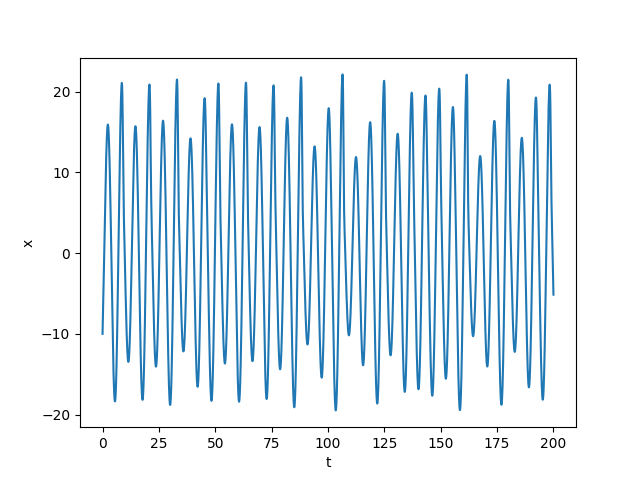
\includegraphics[scale=0.45]{real_trajectory_rossler} 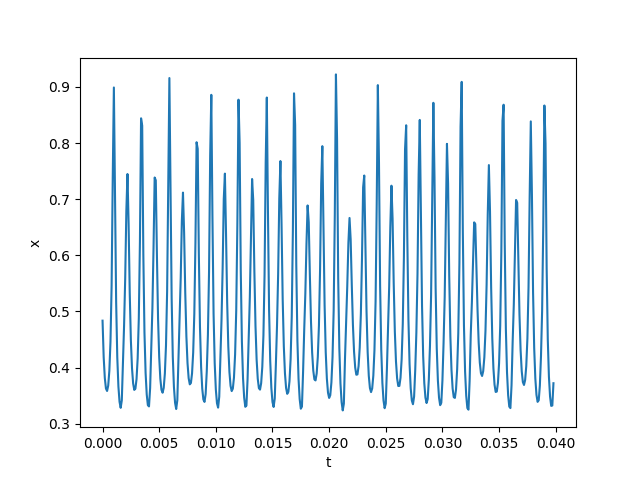
\includegraphics[scale=0.45]{reconstructed_trajectory_rossler}
\caption{Deterministic trajectory for the Rossler attractor in $2d$ (left) and the same plot but reconstructed from the ISIs.}
\label{fig:rossler_xprima}
\end{figure}

From the interspike intervals we define the vectors $(t_i,t_{i+1},t_{i+2})$. This allows us to reconstruct again the phase portrait for the Rossler in $3d$ attractor by connecting the new defined vectors. Note that for all the reconstructions, the only granted preserved feature is the topology, so it's expected for other features such as the scale to be modified. Anyway, if we look at Figure 3, we can appreaciate that some information is preserved as the figure is similar the Rossler attractor and not like any random figure.

\begin{figure}[h!]
\centering
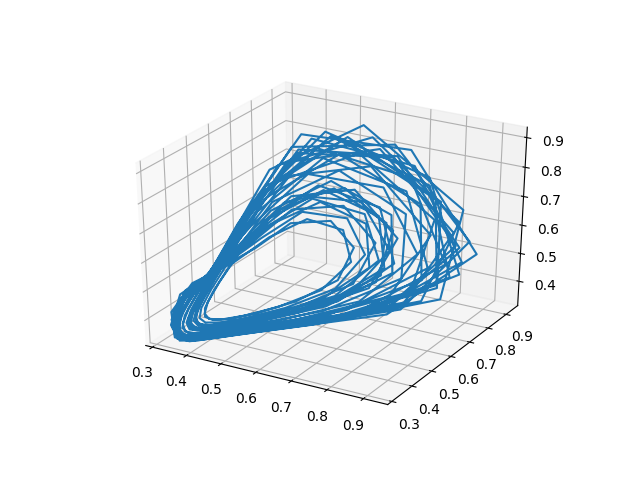
\includegraphics[scale=0.45]{rossler_atractor_400points}
\caption{Reconstruction of the Rossler attractor in $3d$ using our ISIs series with $400$ vectors.}
\label{fig:rossler_isi}
\end{figure}

We can do the same analysis for the Lorentz equations. Although the geometry in the phase portrait is not conserved and we won't plot it as it isn't of any interest, the topology stills and the analysis still valid. Then, we proceed to use the information stored in the ISIs series to unveil the topology of the dynamical system.

\begin{figure}[h!]
\centering
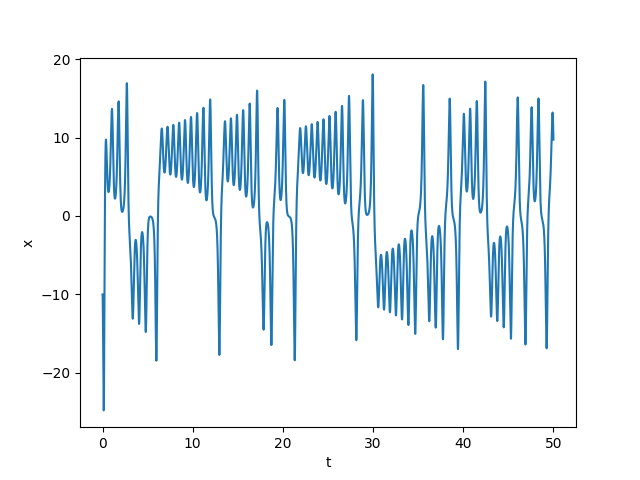
\includegraphics[scale=0.5]{real_trajectory_lorentz}
\caption{Deterministic trajectory from equations described above for the Lorentz system.}
\label{fig:lorentz_trajectory}
\end{figure}

We use the signal $S(t)=(x(t)+2)^2$ and different thresholds used in \cite{interspike} to do the analysis of the prediction error algorithm described in the paper. We basically compare to different methods to predict the expected value for the next time, one of the methods is a k-nearest neighbour and the other is just and averate. As we know that the k-nearest neighbour performs better, we expect for a non-random distribution to have less error in the k-nearest neighbour algorithm than in the average (in fact, it can be proved that for random distributions the average value would perform better). We use this idea of comparing \textit{effectiveness} of algorithms in order to show that we do preserve the information in the process described in the previous sections. 

Then, to be able to compare the results and test our idea of algorithm \textit{effectiveness}  we create surrogate data \cite{surrogate} and plotted with the non-shuffled one in Figure 5. We use the Gaussian-scaled shuffle (GS) surrogate, which is a random shuffle of the original series to preserve the amplitud of the noise but to eliminate any possible temporal correlation more than the one of GS. The GS surrogate corresponds to the null hypothesis that the series is a monotonically scaled version of amplitudes produced by a Gaussian random process. We fix the embedding dimension $m=3$ and predicted one step ahead $(h=1)$, for increasing thresholds $\Theta$, in order to see that the predictability of the series decrease, and tends to disappear as the threshold is big enough.

\begin{figure}[h!]
\centering
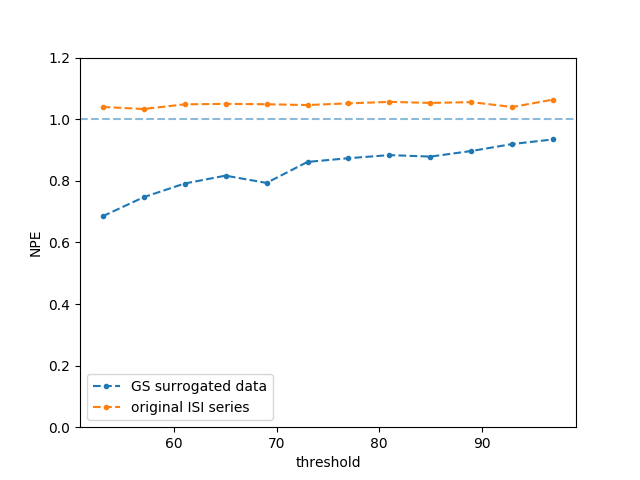
\includegraphics[scale=0.5]{NPE_12series_copy}
\caption{Normalized one step ahead prediction error for several ISI series with varying $\Theta$, for the original ISI series and the GS surrogate.}
\label{fig:12series}
\end{figure}

Finally, as a last result, we reproduce the figure in which they change the step of predictability in order to see how \textit{far} the limit of predictability is and more important to see that there's one in fact, if there wasn't we would be doing something really wrong. We do plot in Figure 6 the predictability for different time advances where we can clearly appreciate that as we increase the number of steps ahead in time the predictability becomes smaller and smaller until a point that there's none unconditioned of the algorithm using. So yes, we can predict in some advance but it doesn't take long for chaos to strike back. This is due to the Liapunov time, or the Liapunov exponent, that tells us when nearby trajectories will diverge thus constrining our limit of predictability

\begin{figure}[h!]
\centering
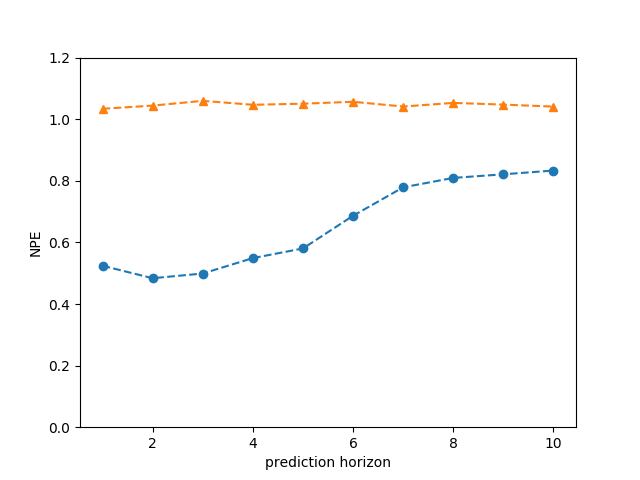
\includegraphics[scale=0.5]{prediction}
\caption{Prediction horizon for ISI's created by the Lorentz attractor with $S(t)=(x+y+z)^2$ and $\Theta = 200$ (circles) and the same for Gaussian Shuffle (triangles). }
\label{fig:distributions}
\end{figure}

\section{Conclusions}
Although confusing at first glance as the principal ideas are counter intuitive, we found here an interesting application to time series. We consider, nevertheless, that there is a lack of mathematical fundament in both papers, although the second one relies explicitly on Takens's theorem, it seems to need some general analysis. We realize how powerful this procedures explained above can be, since with little information of a dyamical system we can extract the main characteristics, reconstructing some shape of the attractor of the underlying system, establish wheter it is deterministic or stochastic, with a prediction algorithm, and even to make predictions of the future evolution, with different step-ahead. We succeeded in obtaining the main results, such that we acquired a good understanding of these topics.

\begin{thebibliography}{99}
 
\bibitem{paper1}N. H. Packard, J. P. Crutchfield, J. D. Farmer, and R. S. Shaw, {\it Geometry from a Time Series}, Dynamical Systems Collective, Physics DePartment, University of California, Santa Crae, California (13 November 1979).

\bibitem{interspike}Tim Sauer, {\it Reconstruction of Dynamical Systems from Interspike Intervals}, Department of Mathematical Sciences, Geode Mason University, Fairfas, Vinpnia (Received 15 February 1994).

\bibitem{takens}F. Takens, {\it Dynamical Systems and Turbulence}, Lecture Notes in Math-
ematics Vol. 898 (Springer-Verlsg, Berlin, 1981).

\bibitem{surrogate}J. Theiler, S. Eubank, A. Longtin, B. Gsldrakian, and
J. D. Farmer, Physics (Amsterdam) 58D, 77 (1992).

\end{thebibliography}

\end{document}